\documentclass[a4paper,14pt]{extreport}
\usepackage[left=1.5cm,right=1.5cm,
    top=1.5cm,bottom=2cm,bindingoffset=0cm]{geometry}
\usepackage{scrextend}
\usepackage[T1,T2A]{fontenc}
\usepackage[utf8]{inputenc}
\usepackage[english,russian,ukrainian]{babel}
\usepackage{tabularx}
\usepackage{amssymb}
\usepackage{color}
\usepackage{amsmath}
\usepackage{mathrsfs}
\usepackage{listings}
\usepackage{graphicx}
\graphicspath{ {./images/} }
\usepackage{lipsum}
\usepackage{xcolor}
\usepackage{hyperref}
\usepackage{tcolorbox}
\usepackage{tikz}
\usepackage[framemethod=TikZ]{mdframed}
\usepackage{wrapfig,boxedminipage,lipsum}
\mdfdefinestyle{MyFrame}{%
linecolor=blue,outerlinewidth=2pt,roundcorner=20pt,innertopmargin=\baselineskip,innerbottommargin=\baselineskip,innerrightmargin=20pt,innerleftmargin=20pt,backgroundcolor=gray!50!white}
 \usepackage{csvsimple}
 \usepackage{supertabular}
\usepackage{pdflscape}
\usepackage{fancyvrb}
%\usepackage{comment}
\usepackage{array,tabularx}
\usepackage{colortbl}

\usepackage{varwidth}
\tcbuselibrary{skins}
\usepackage{fancybox}


\usepackage{tikz}
\usepackage[framemethod=TikZ]{mdframed}
\usepackage{xcolor}
\usetikzlibrary{calc}
\makeatletter
\newlength{\mylength}
\xdef\CircleFactor{1.1}
\setlength\mylength{\dimexpr\f@size pt}
\newsavebox{\mybox}
\newcommand*\circled[2][draw=blue]{\savebox\mybox{\vbox{\vphantom{WL1/}#1}}\setlength\mylength{\dimexpr\CircleFactor\dimexpr\ht\mybox+\dp\mybox\relax\relax}\tikzset{mystyle/.style={circle,#1,minimum height={\mylength}}}
\tikz[baseline=(char.base)]
\node[mystyle] (char) {#2};}
\makeatother

\definecolor{ggreen}{rgb}{0.4,1,0}
\definecolor{rred}{rgb}{1,0.1,0.1}
\definecolor{amber}{rgb}{1.0, 0.75, 0.0}
\definecolor{babyblue}{rgb}{0.54, 0.81, 0.94}
\definecolor{amethyst}{rgb}{0.6, 0.4, 0.8}

\usepackage{float}
\usepackage{wrapfig}
\usepackage{framed}
%for nice Code{
\lstdefinestyle{customc}{
  belowcaptionskip=1\baselineskip,
  breaklines=true,
  frame=L,
  xleftmargin=\parindent,
  language=C,
  showstringspaces=false,
  basicstyle=\small\ttfamily,
  keywordstyle=\bfseries\color{green!40!black},
  commentstyle=\itshape\color{purple!40!black},
  identifierstyle=\color{blue},
  stringstyle=\color{orange},
}
\lstset{escapechar=@,style=customc}
%}


\begin{document}
\pagecolor{white}

%----------------------------------------1
\newtcbox{\xmybox}[1][red]{on line, arc=7pt,colback=#1!10!white,colframe=#1!50!black, before upper={\rule[-3pt]{0pt}{10pt}},boxrule=1pt, boxsep=0pt,left=6pt,right=6pt,top=2pt,bottom=2pt}

\begin{titlepage}
  \begin{center}
    \large
    Національний технічний університет України \\ "Київський політехнічний інститут імені Ігоря Сікорського"


    Факультет Електроніки

    Кафедра мікроелектроніки
    \vfill

    \textsc{ЗВІТ}\\

    {\Large Про виконання лабораторної роботи №1\\
      з дисципліни: «Схемотехніка-1»\\[1cm]

        ПІДСИЛЮВАЧІ НА БІПОЛЯРНИХ ТРАНЗИСТОРАХ


    }
  \bigskip
\end{center}
\vfill

\newlength{\ML}
\settowidth{\ML}{«\underline{\hspace{0.4cm}}» \underline{\hspace{2cm}}}
\hfill
\begin{minipage}{1\textwidth}
Виконавець:\\
Студент 3-го курсу \hspace{4cm} $\underset{\text{(підпис)}}{\underline{\hspace{0.2\textwidth}}}$  \hspace{1cm}Б.\,В.~Лищенко\\
\vspace{1cm}

Перевірила: \hspace{6.1cm} $\underset{\text{(підпис)}}{\underline{\hspace{0.2\textwidth}}}$  \hspace{1cm}Г.\,С.~Порева\\

\end{minipage}

\vfill

\begin{center}
2021
\end{center}
\end{titlepage}

    %----------------------------------------
  %--------------     1     ---------------
%----------------------------------------

\newpage
\setcounter{page}{2}

\textbf{Мета роботи:} Вивчення принципів роботи, дослідження амплітудних та частотних характеристик і параметрів підсилювачів на основі біполярних транзисторів (зі Спільним Емітером (СЕ), Спільним Колектором (СК), Спільною Базою(СБ)).



\begin{figure}[h]
\center{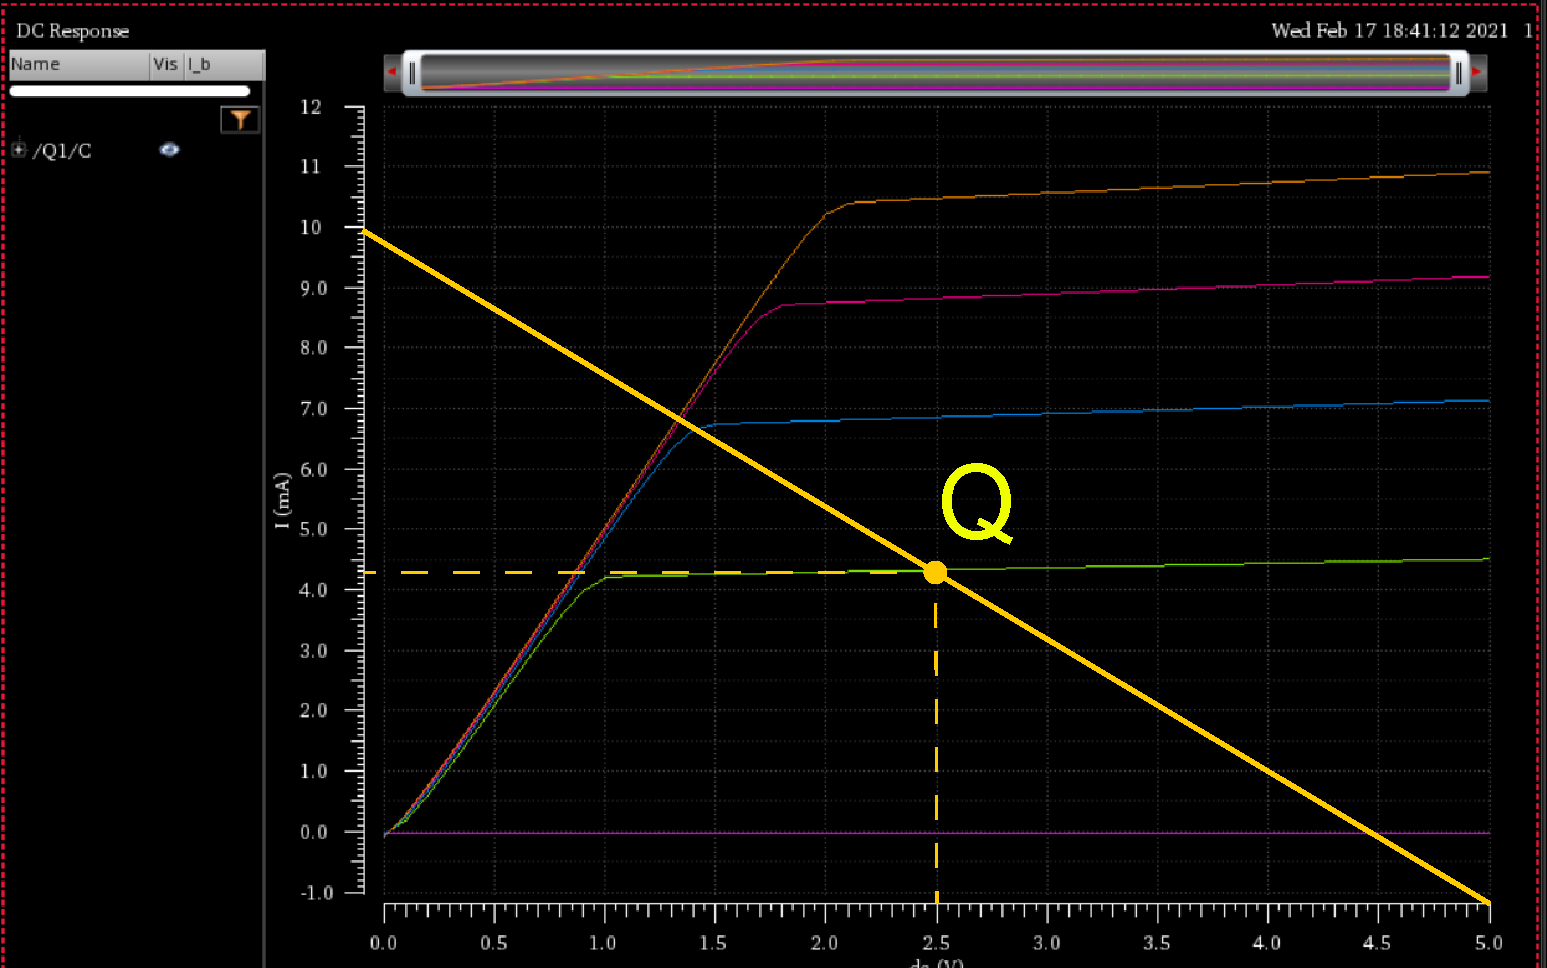
\includegraphics[width=1\linewidth]{1.png}}
\caption{Блок-схема установки для дослідження лабораторного модуля «ПБТ».}
\label{ris1}
\end{figure}
Лабораторна установка для дослідження лабораторного модуля «ПБТ» складається з генератора гармонічних коливань 1 типу Г3-112, лабораторного стенду 2 типу «Каскад М», вольтметрів 3 і 5 типу В3-38, осцилографа 4 типу С1-55, магазину опорів 6. До складу лабораторного стенду 2 входять стабілізований блок живлення, електронний комутатор, формувач імпульсів, чотири лабораторних модулі.\par
Генератор 1 є джерелом гармонійної вихідної напруги в частотному діапазоні від 20 Гц до 1 МГц та амплітудою від 0 до 6,3 В.\par
Вольтметри 3 та 5 призначені для вимірювання амплітуди відповідно вхідної U1 та вихідної U2 напруги від 0,1 мВ до 200 В у діапазоні частот від 20 Гц до 3 МГц.\par
Осцилограф 4 використовується для спостереження на екрані електронно-променевої трубки форми напруги та вимірювання параметрів напруги від 30 мВ до 140 В у частотному діапазоні від 3 Гц до 10 МГц.\par
Магазин опорів 6 забезпечує вибір необхідного опору.

\begin{figure}[h]
\center{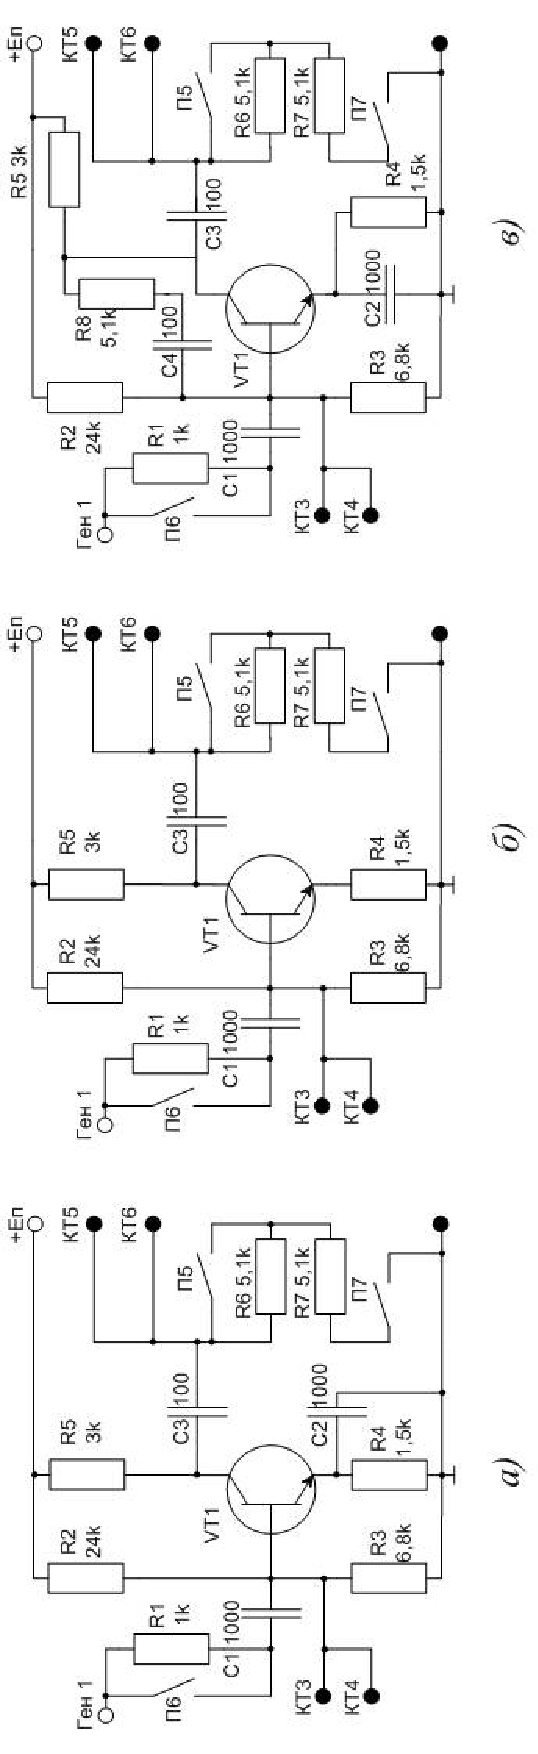
\includegraphics[angle=-90, width=1\linewidth]{1.1.pdf}}
\label{ris5}
\caption{Схема електрична принципова лабораторного модуля «ПБТ»:
а) схема зі спільним емітером (П1-вкл), б) схема зі спільною базою
(П2-вкл), в) схема зі спільним колектором (П3-вкл).}
\end{figure}


    %----------------------------------------
  %--------------     2     ---------------
%----------------------------------------

\begin{figure}[h]
\center{\includegraphics[width=0.7\linewidth]{1.2.png}}
\label{ris6}
\caption{Реалізовані в лабораторному модулі схеми.}
\end{figure}


\begin{figure}[h]
До вимірюванню функцій підсилювачів.
\center{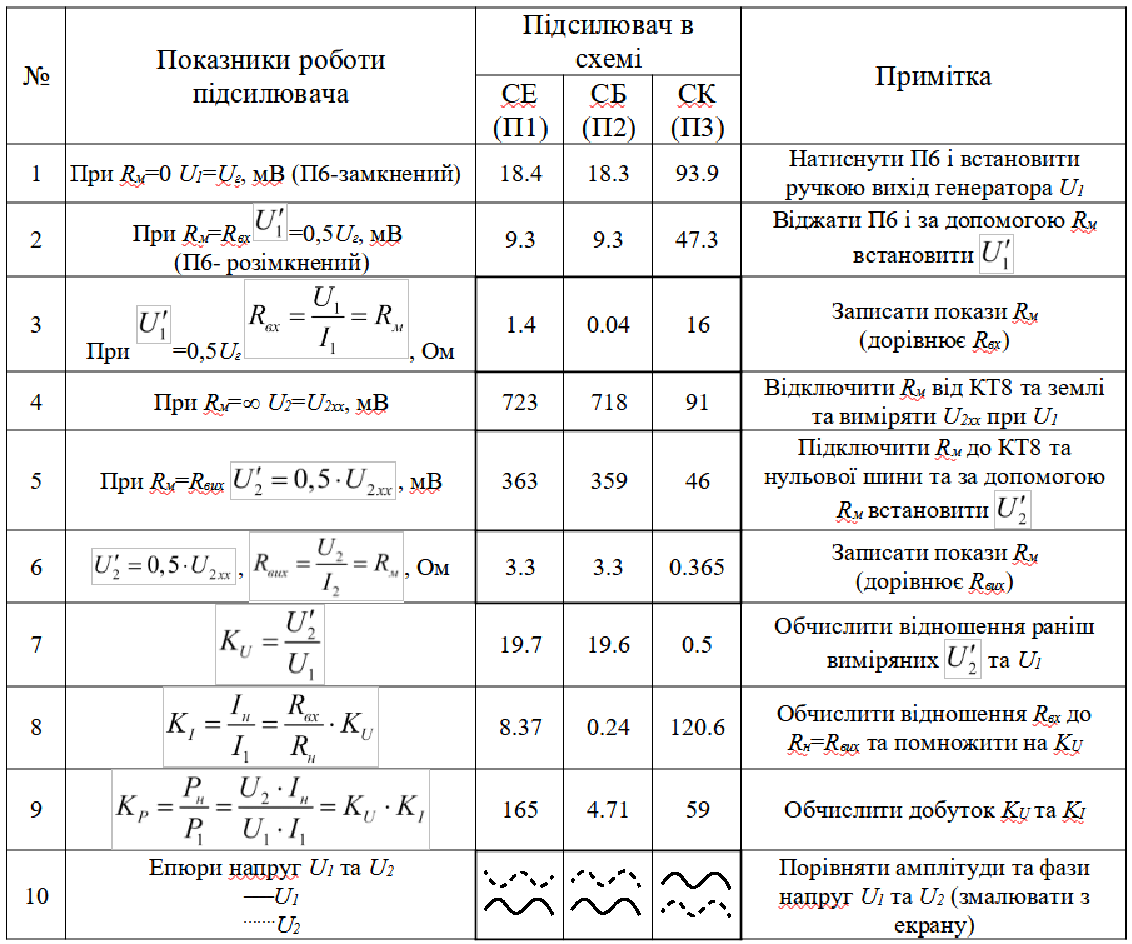
\includegraphics[width=1\linewidth]{t1.pdf}}
\label{ris2}
\end{figure}

\clearpage
\begin{figure}[h]
До вимірюванню амплітудних характеристик підсилювача
\center{\includegraphics[width=0.7\linewidth]{t2.png}}
\label{ris3}
\end{figure}

\begin{figure}[h]
\center{\includegraphics[width=0.7\linewidth]{r1.png}}
\label{ris31}
\caption{Амплытудні хар-ки підсилювачів в схемі СЕ, СБ, СК.}
\end{figure}


\begin{figure}[h]
До вимірюванню частотних характеристик підсилювача.
\center{\includegraphics[width=0.6\linewidth]{t3.png}}
\label{ris4}
\end{figure}


\begin{figure}[h]
\center{\includegraphics[width=0.6\linewidth]{r11.png}}
\label{ris5}
\caption{АЧХ у нормованому вигляді в схемі СЕ, СБ, СК.}
\end{figure}

\clearpage
\newpage

\begin{center}ВИСНОВКИ\end{center}
Аналізуючи результатам цієї лабораторної роботи, можна сказати, що найбільший коефіцієнт підсилення по напрузі та потужності має схема зі спільним емітером в якій відбувається зсув фаз на 180$^\circ$ відносно вхідного сигналу, а схема зі спільним колектором має найбільший коефіціетн підсилення за струмом і має найбільший діапазон робочих частот порівняно з іншими схемами.
















\end{document}
